\chapter{Campos vectoriales}

Los comandos usados para representar campos vectoriales son \textbf{quiver} y \textbf{quiver3}, que son respectivamente para 2D y 3D. Básicamente, a cada punto se le asigna un vector y se lo representa. Veamos un ejemplo:

\begin{lstlisting}[language=Matlab]
>> [X,Y] = meshgrid(-2:.15:2,-2:.15:2);
>> Z = X.*exp(-X.^2-Y.^2);
>> [px,py] = gradient(Z,.15,.15);
>> contour(X,Y,Z), hold on, quiver(X,Y,px,py), colorbar
>> hold off
\end{lstlisting}

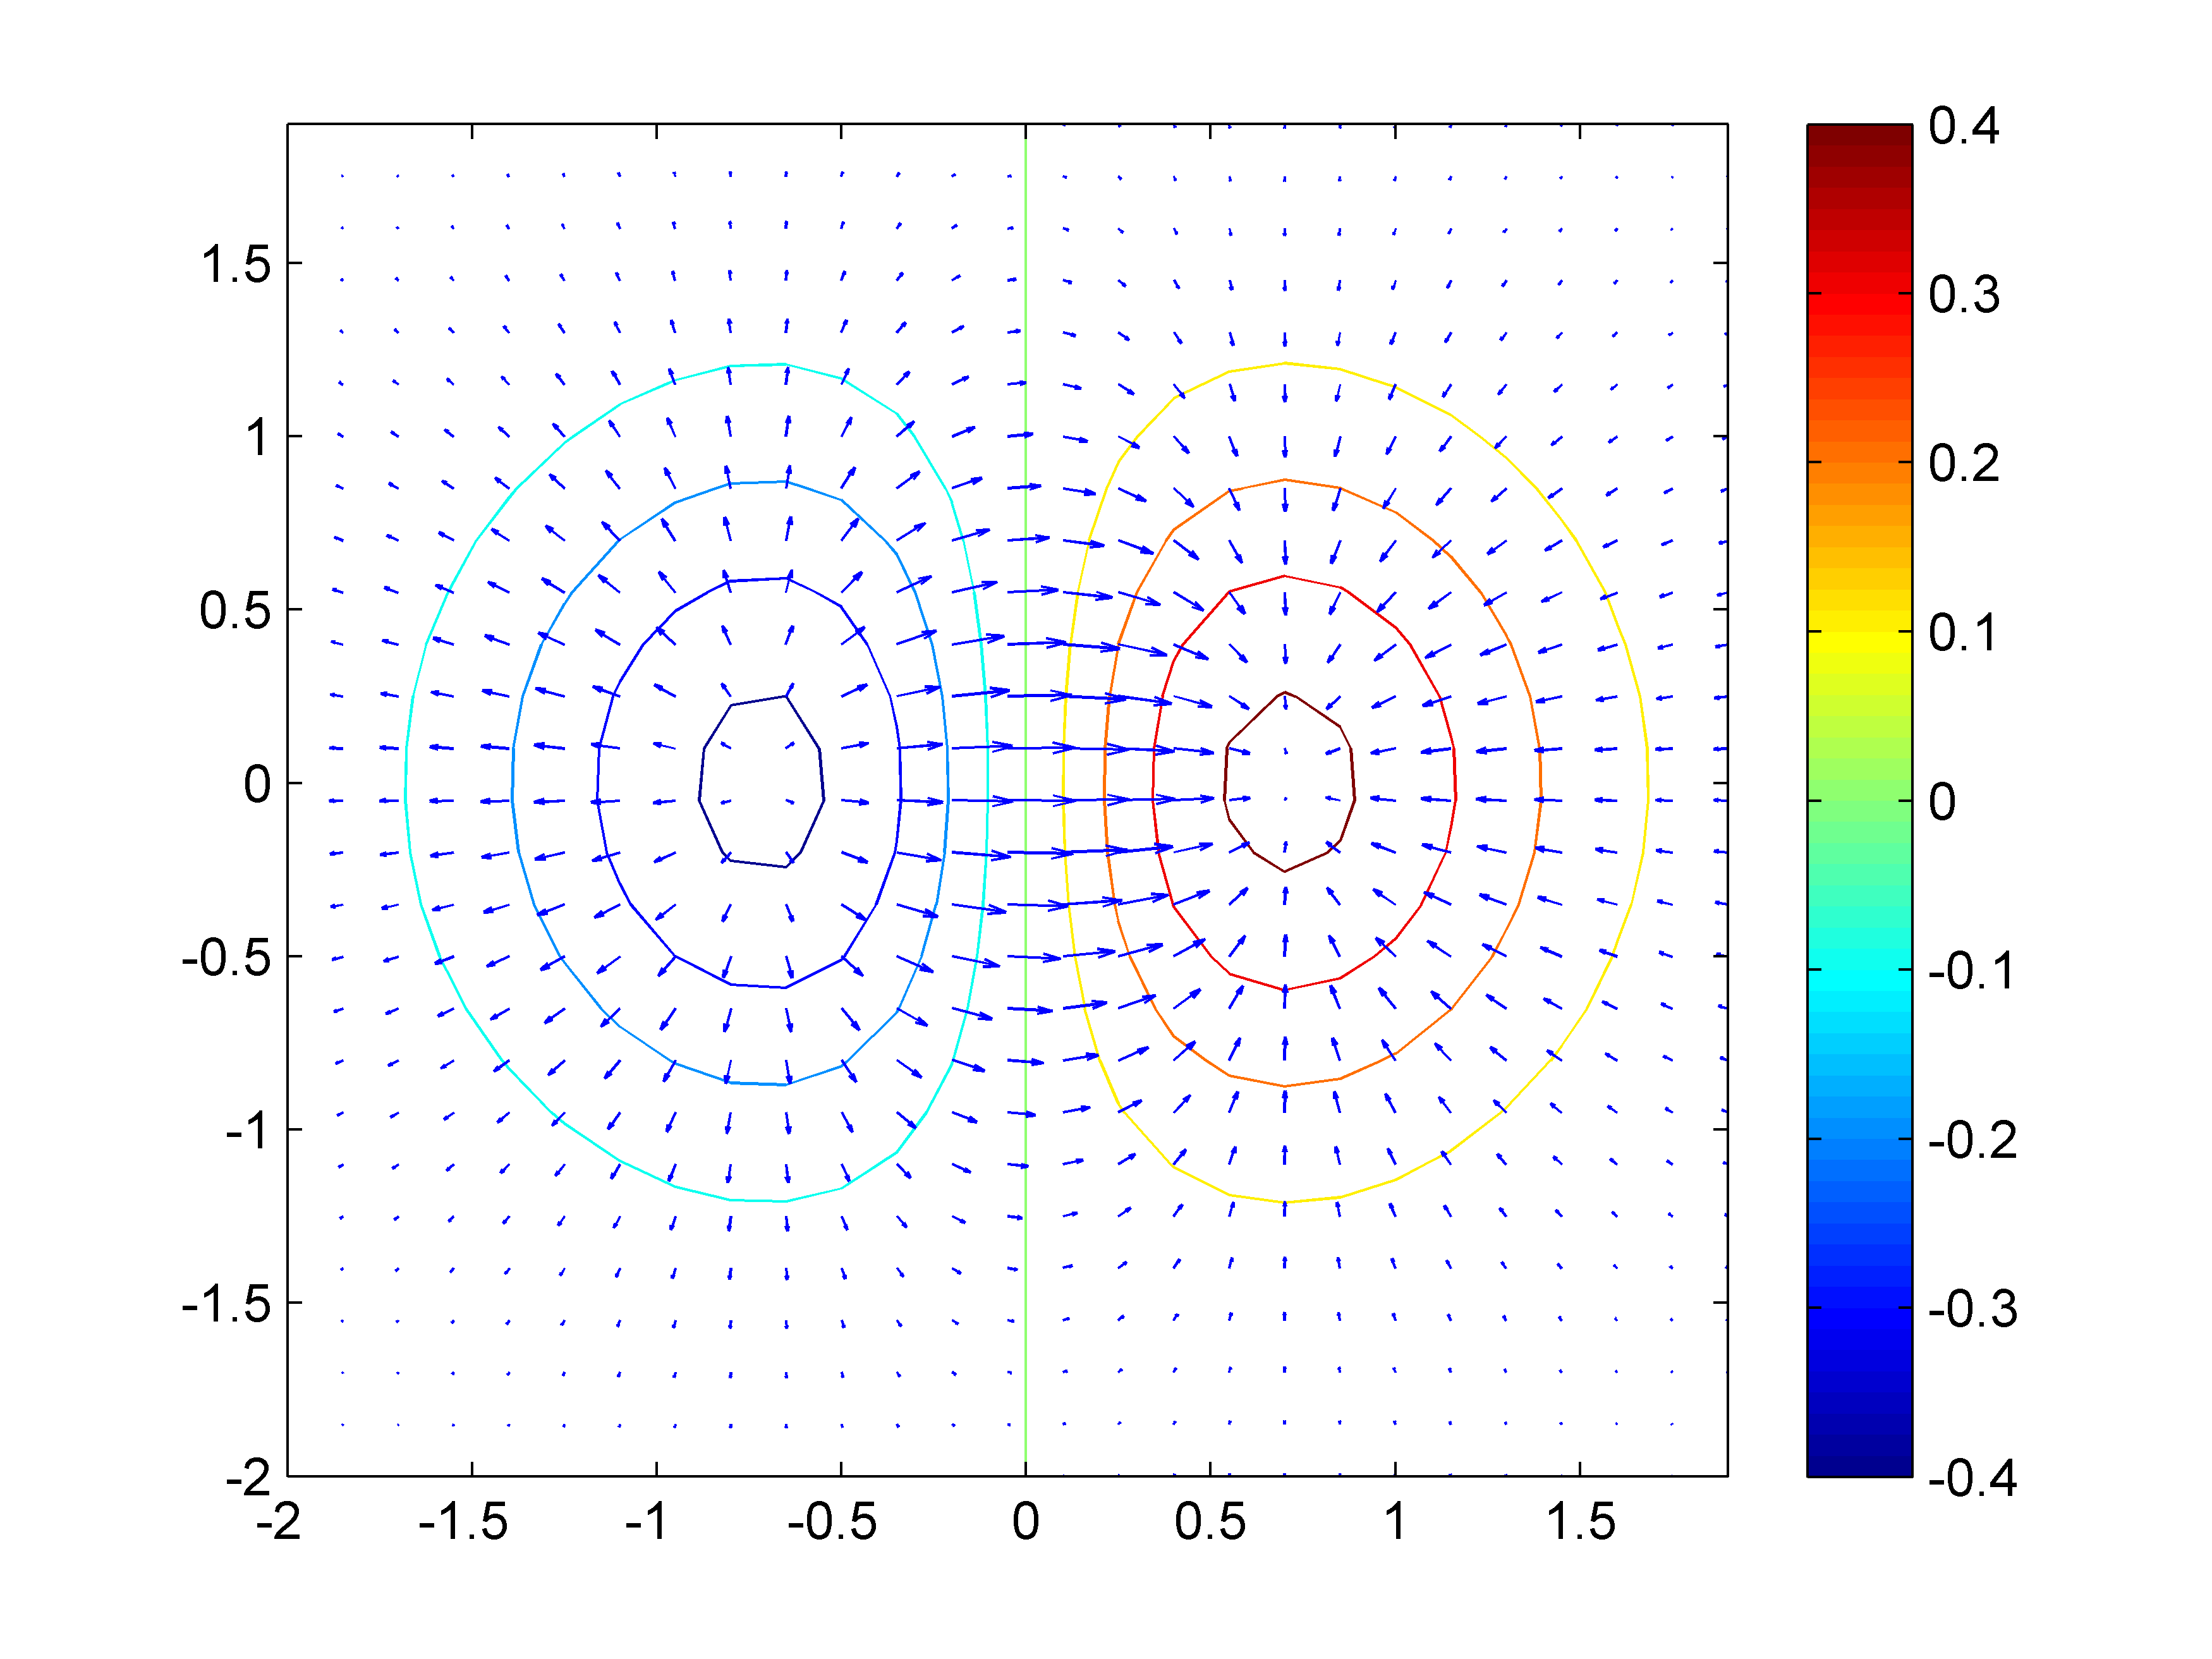
\includegraphics[width=400pt]{./Imagenes/cvector1.png}

Otro ejemplo podemos verlo con los campos vectoriales gradientes. Para ellos conviene utilizar la orden $[px,py]=gradient(f,hx,hy)$, que calcula una aproximación por diferencias al gradiente de f, utilizando $hx$, $hy$ como los desplazamientos en las direcciones de abscisas y ordenadas respectivamente, según las formulas:
\begin{center}
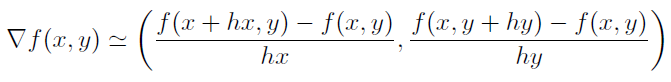
\includegraphics[width=300pt]{./Imagenes/grad.png}
\end{center}

Vamos a ver otro ejemplo. Para representar un campo vectorial, primero definimos las funciones componentes del campo, luego las restricciones para las variables que definen F, construir las matrices X e Y, finalmente con \textbf{quiver} dibujar el campo.

\begin{lstlisting}[language=Matlab]
>> u=inline('0*x+1','x','y'); 
>> v=inline('x+y.^2','x','y'); 
>> x=linspace(-2,3,11); 
>> y=linspace(-1,2,11); 
>> [X,Y]=meshgrid(x,y); 
>> U=u(X,Y);V=v(X,Y); 
>> quiver(X,Y,U,V) 
>> axis image 
\end{lstlisting}

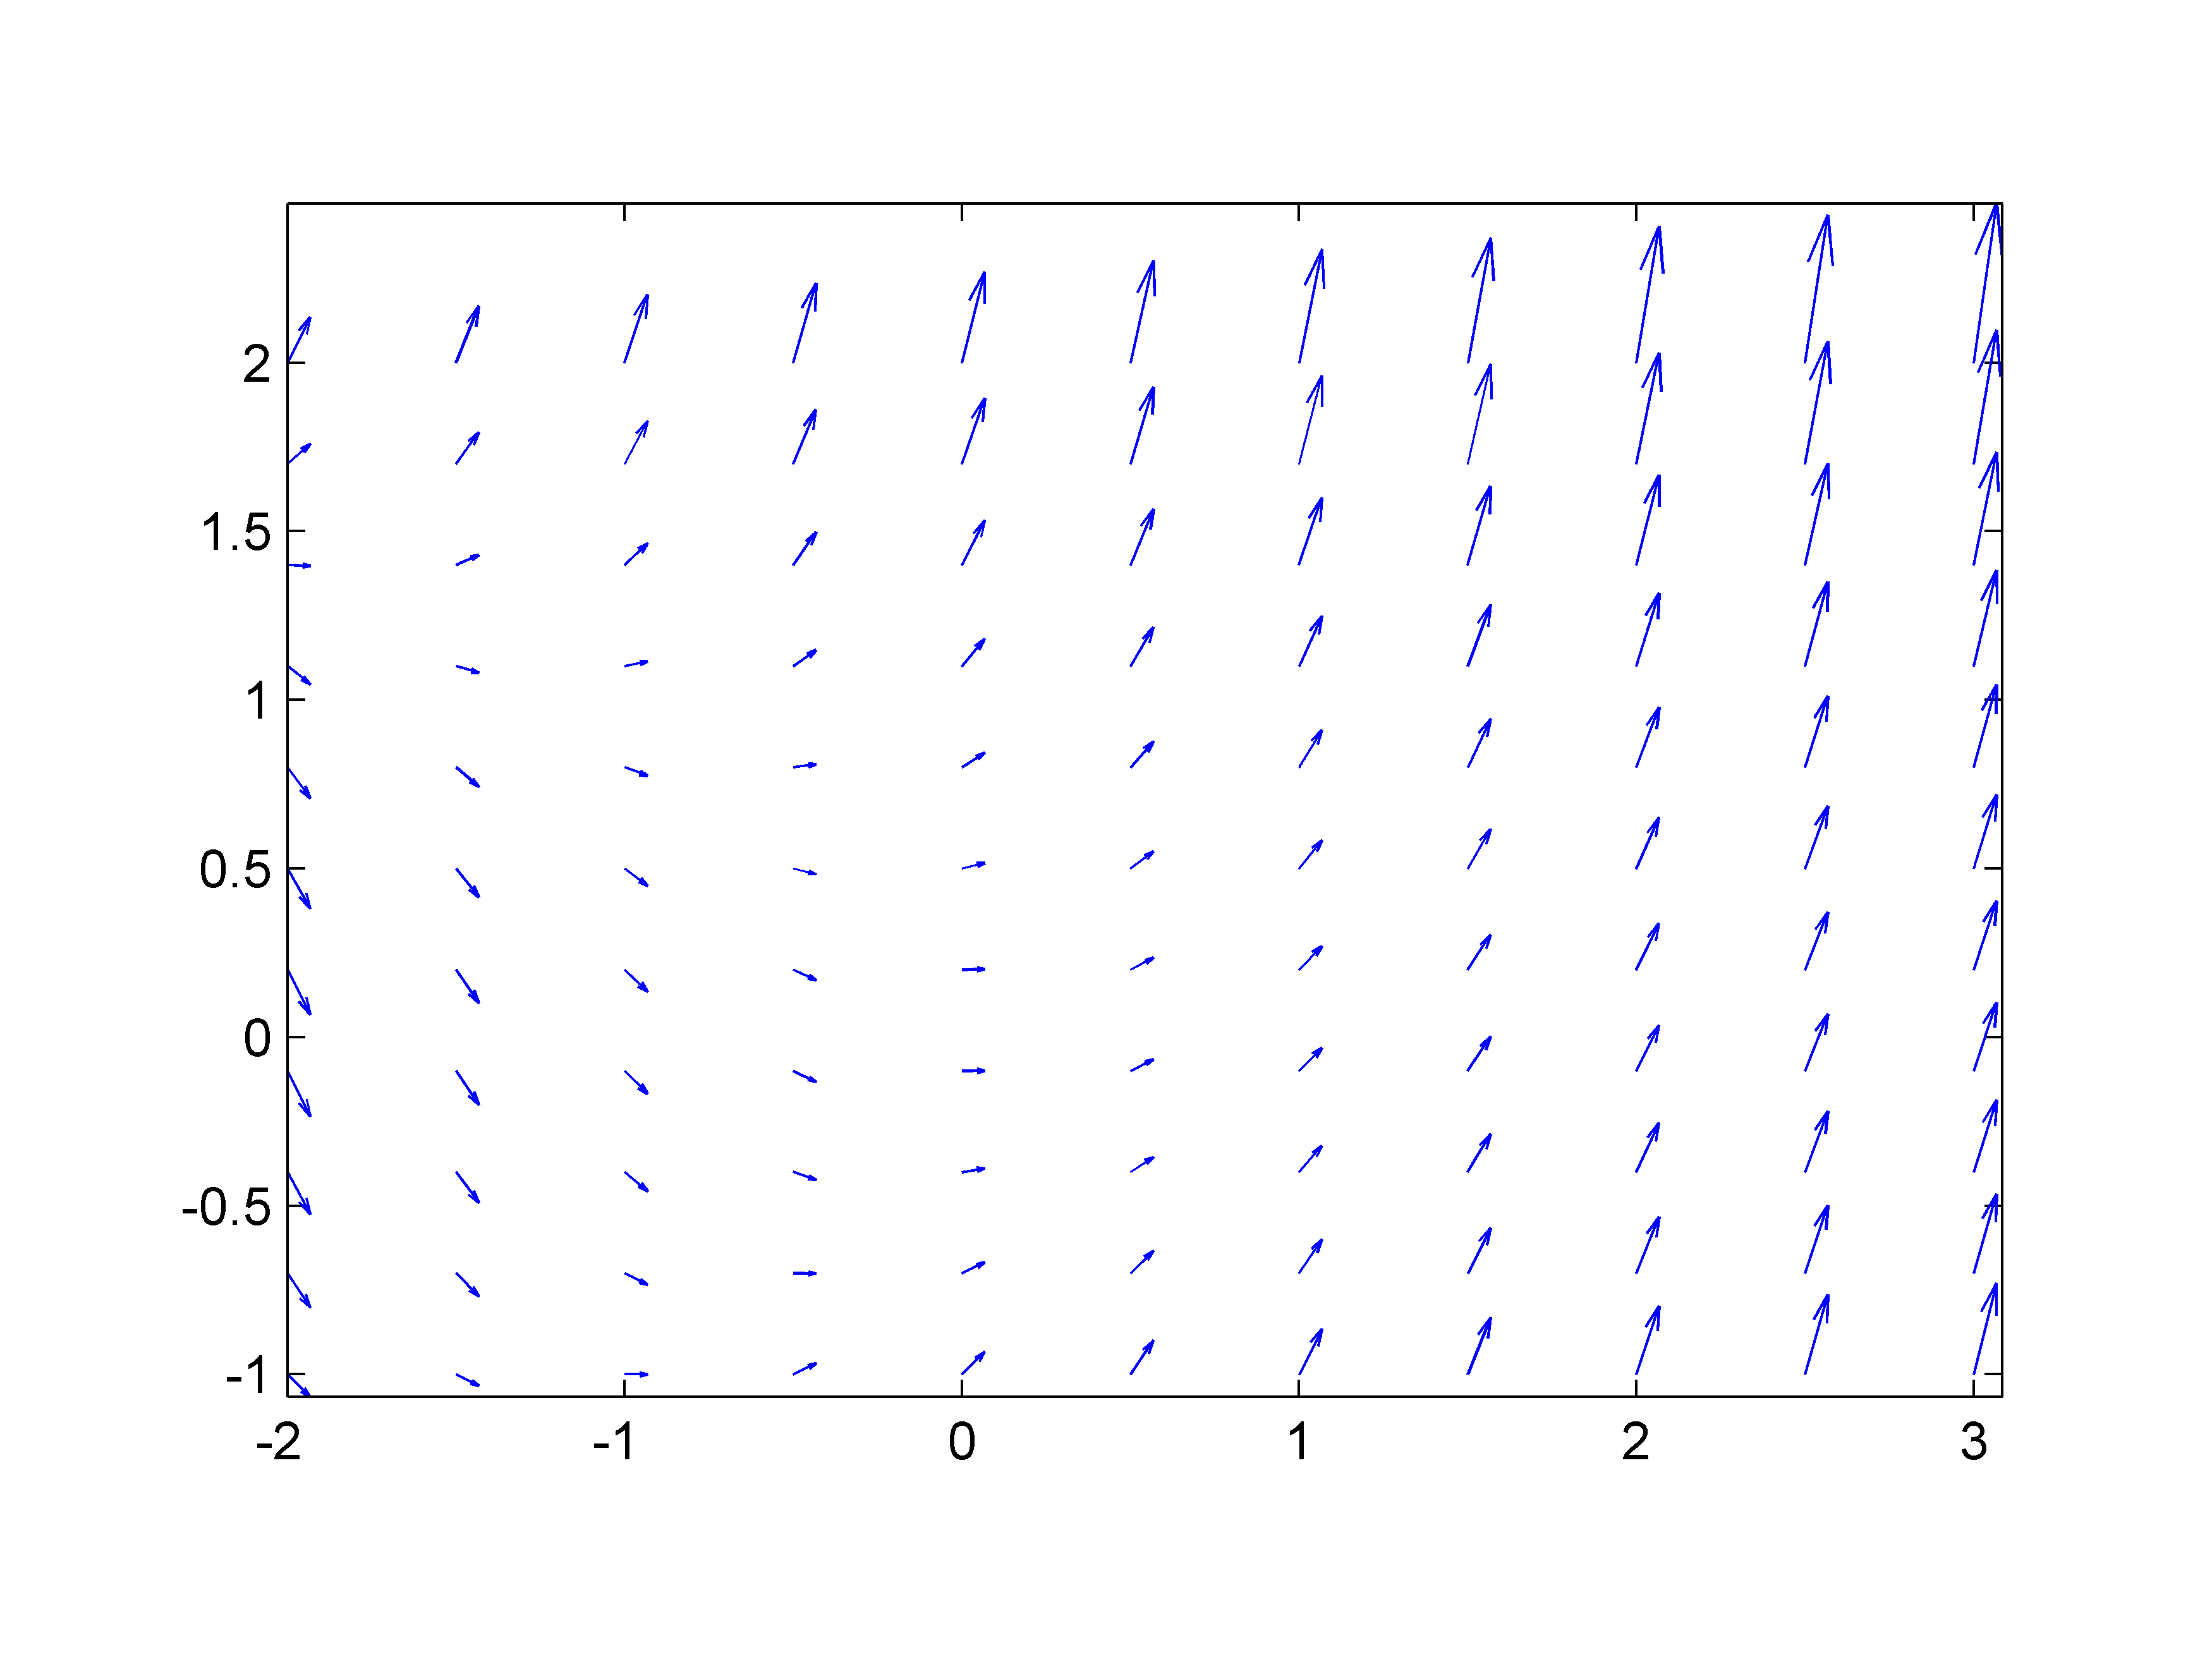
\includegraphics[width=400pt]{./Imagenes/vectorial1.png}